% Resource and auditor trace figures for the ten annotated runs. Built by
% figures/app_H2.py from the run transcripts; see the comment block at the
% top of h_runs.tex for the data of record. Compute charged is budget_h100
% minus remaining_h100 after each call, normalised by the record's spent_h100,
% which is also the figure printed at right; the event stream's last
% remaining_h100 falls short of it in runs 5 and 7, so those two areas stop
% below the lane top. Wall-clock is t_rel_s normalised by the run's last
% timestamp. The auditor strip classifies each audit_events call by the path
% it opened or the command it ran; the rule and the per-call classification
% print with app_H2.py --dump. It draws the classes in four colors the paper
% already uses, so they do not read as the Appendix G failure-mode colors.

% h_runs.tex pulls this file in after the tenth vignette, so these two
% figures close the appendix; the barrier below flushes vignette ten's card
% and panel first, and the barrier after the \input keeps both figures inside
% Appendix H.
\FloatBarrier

Figure~\ref{fig:run-timelines} places the ten runs on one round axis,
colored by what the agent did in each round.
Figure~\ref{fig:app-h2-resource-trace} follows the same runs by the
compute charged and the wall-clock elapsed by round, each as a share of the
run's total, so the reader can see which rounds the budget went to.
Figure~\ref{fig:app-h2-auditor-trace} shows the auditor's own session on
each run, one cell per tool call colored by what it opened or ran, with the
pinned verdict and the flags it raised.

\begin{figure}[p]
\centering
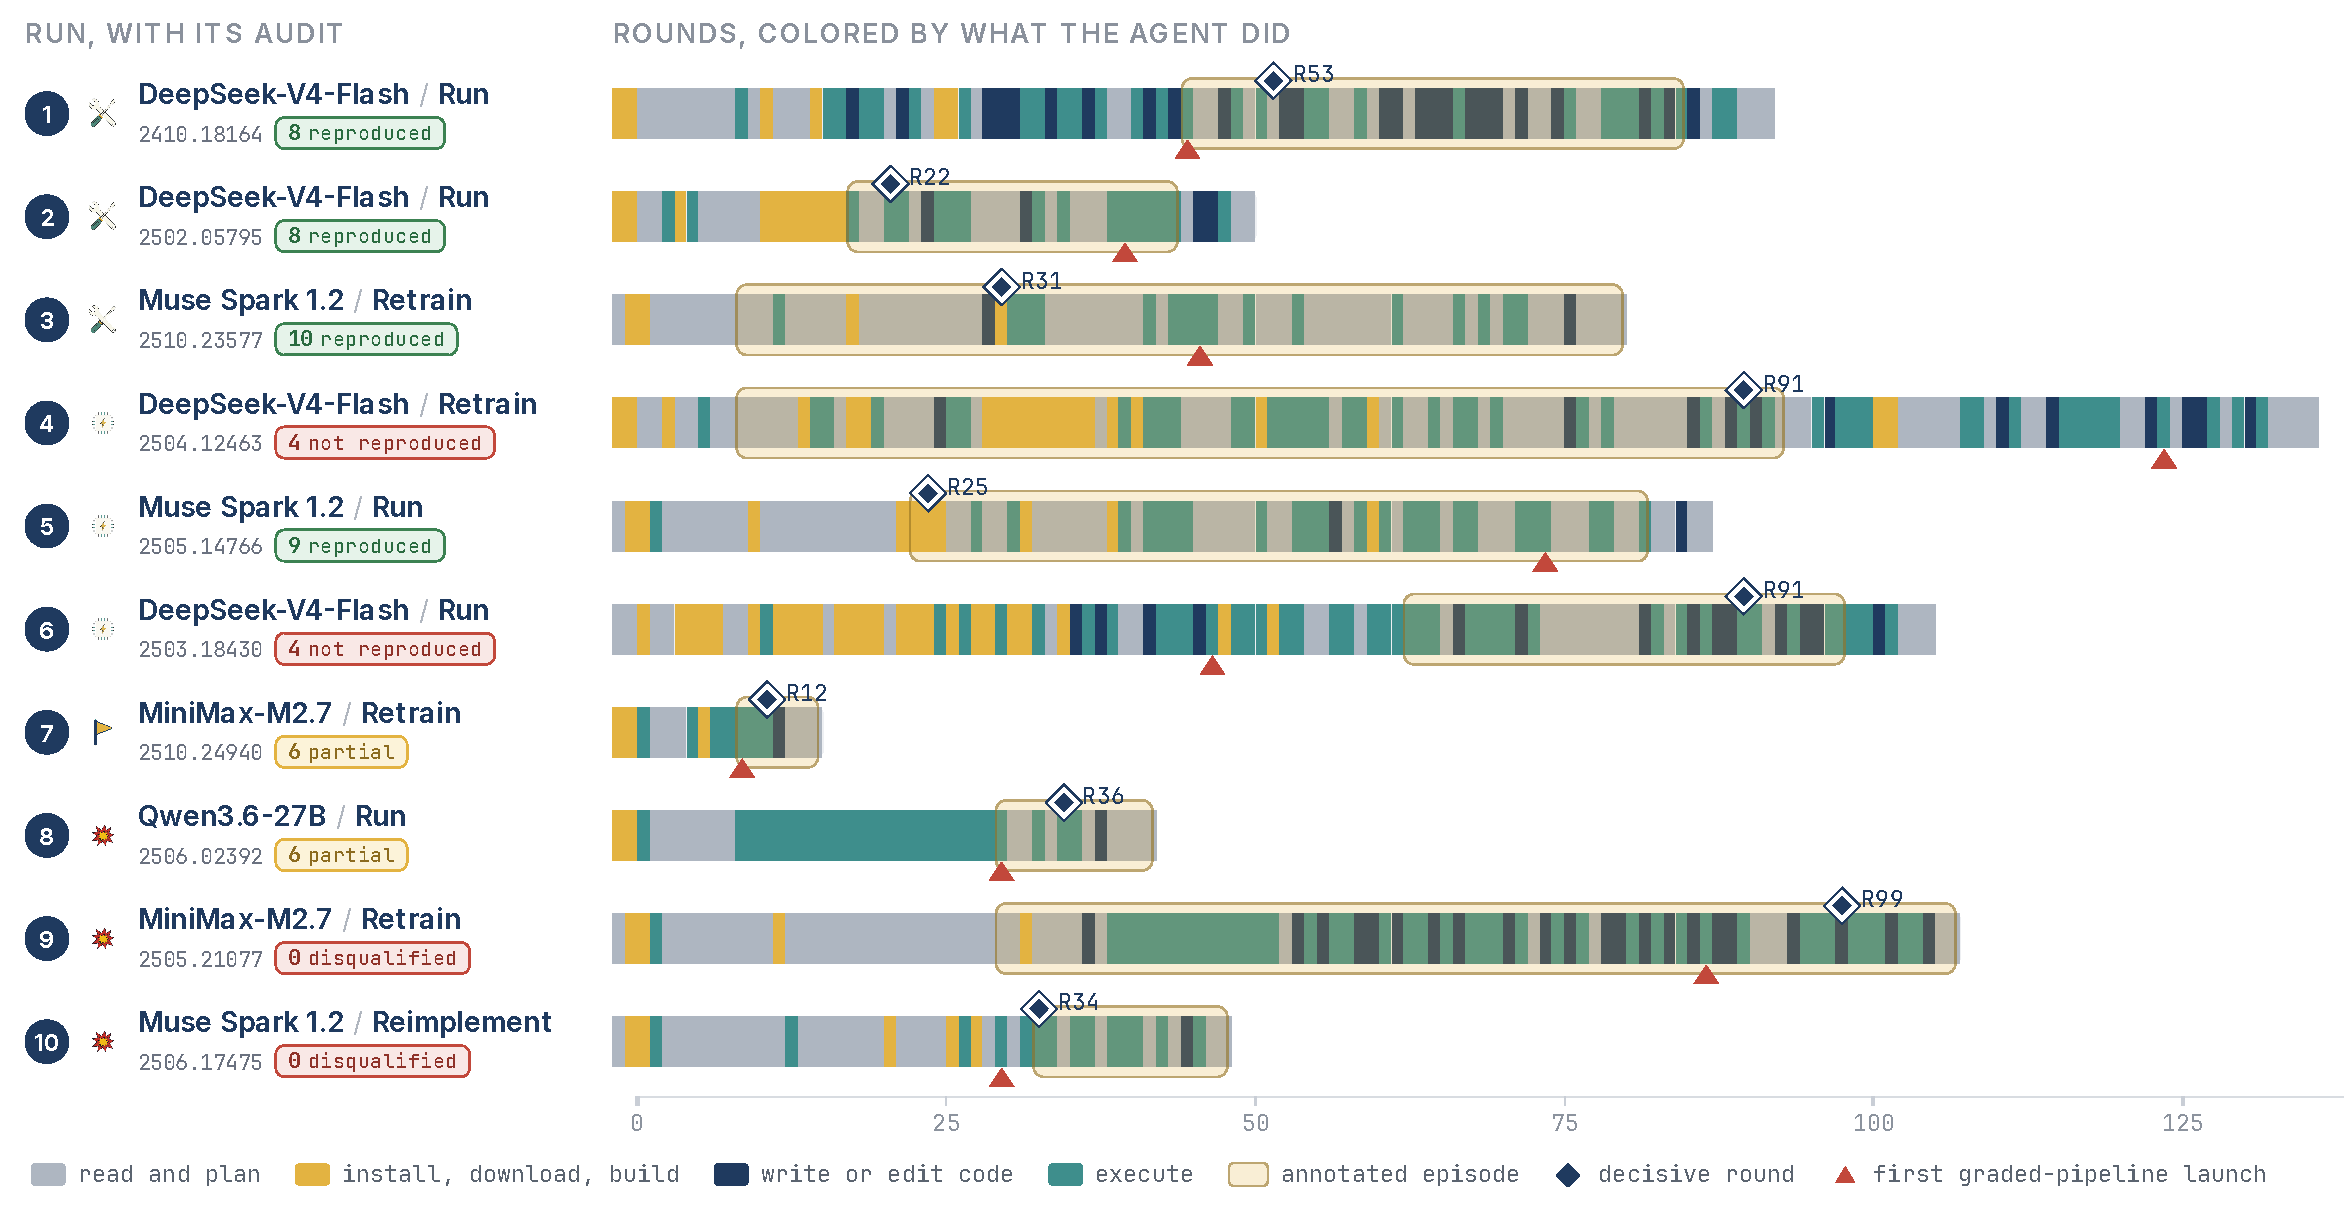
\includegraphics[width=\textwidth]{figures/run_timelines}
\caption{Activity of the ten annotated runs by round, colored by the kind
of tool call, with the annotated episode, its decisive round, and the first
graded-pipeline launch marked.}
\label{fig:run-timelines}
\end{figure}

\begin{figure}[htb]
\centering
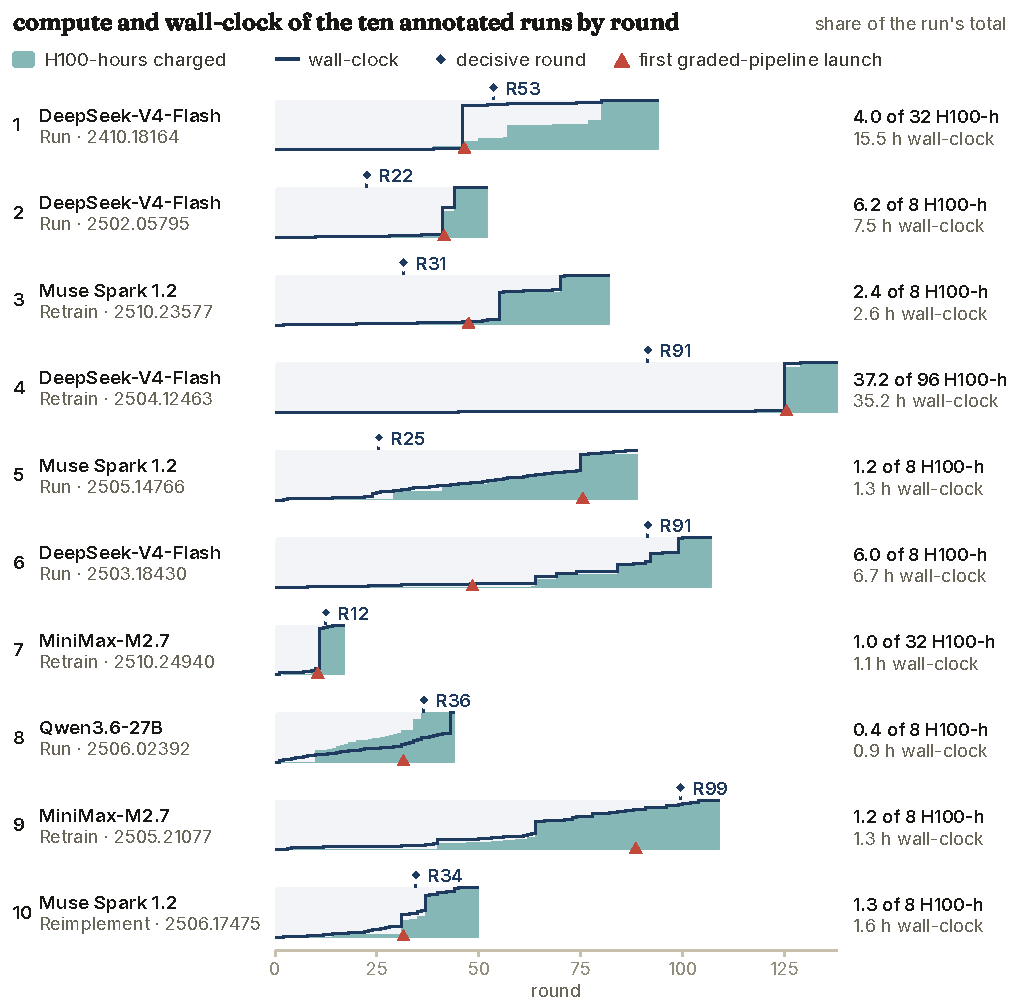
\includegraphics[width=\textwidth]{figures/app_H2_resource_trace}
\caption{Compute charged and wall-clock elapsed by round for the ten
annotated runs, each as a share of the run's total, with the decisive round
and the first graded-pipeline launch marked.}
\label{fig:app-h2-resource-trace}
\end{figure}

\begin{figure}[htb]
\centering
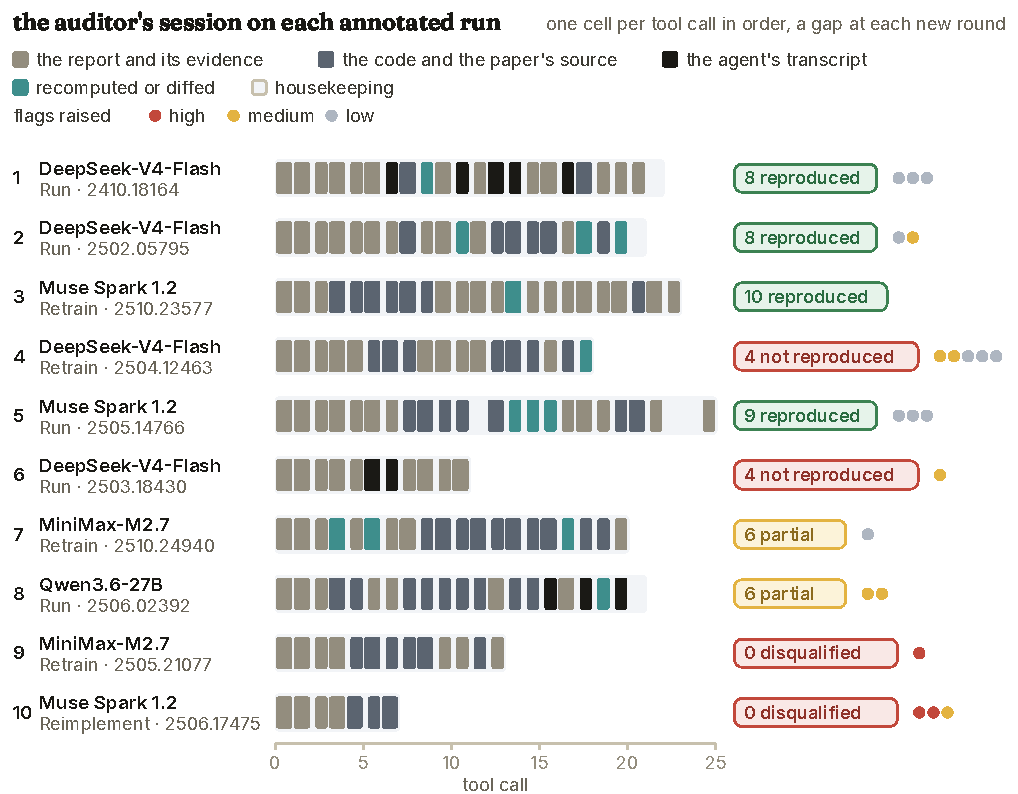
\includegraphics[width=\textwidth]{figures/app_H2_auditor_trace}
\caption{The auditor's session on each of the ten annotated runs, one cell
per tool call in order and colored by what it opened or ran, with the pinned
verdict and the flags it raised.}
\label{fig:app-h2-auditor-trace}
\end{figure}
